%!TEX root = ../thesis.tex


\begin{table}[]
\centering
\resizebox{\textwidth}{!}{%
\begin{tabular}{llll}
\hline
Method                & Description \\ \hline
execCommand           & Executes a command. \\
queryCommandEnabled   & Returns whether or not a given command can currently be executed. \\
queryCommandIndeterm  & Returns whether or not a given command is in the indeterminate state. \\
queryCommandState     & Returns the current state of a given command. \\
queryCommandSupported & Returns whether or not a given command is supported by the current document's range. \\
queryCommandValue     & Returns the value for the given command. \\ \hline
\end{tabular}
}
\caption{HTML Editing API}
\label{table:editing_mode_api}
\end{table}


\clearpage
\newpage


\begin{table}[]
\centering
\resizebox{\linewidth}{!}{%
\begin{tabularx}{\textwidth}{|l|X|}
\hline
Example call    &    Description \\ \hline


type.caret()	&	 Returns the offset of the caret \\
type.caret('show')	&	 Show the caret \\
type.caret('hide')	&	 Hides the caret \\
type.caret(10)	&	 Moves the caret to the 10th character \\
type.caret(10, 20)	&	 Convenience function for type.select(10, 20) \\ \hline

type.selection()	&	 Same as type.selection('text') \\
type.selection('text')	&	 Returns the unformatted (plain) contents of the current selection \\
type.selection('html')	&	 Return the currently selected HTML \\
type.selection(10)	&	 Convenience function for type.caret(10) \\
type.selection(10, 20)	&	 Selects characters 10 to 20 \\
type.selection(element)	&	 Select an element \\
type.selection(element1, element2)	&	 Creates a selection between 2 elements \\
type.selection(jQueryCollection)	&	 Creates a selection between the first and last element in the jQuery Collection \\
type.selection('save')	&	 Returns an object that can be passed to type.selection('restore') to store and recreate a selection \\
type.selection('restore', sel)	&	 Takes an object returned by type.selection('save') as a second argument to recreate a stored selection \\ \hline

type.insert(str)	&	 Inserts plain text at the caret's position, regardless if str contains html. Will overwrite the current	 selection if there is one. \\
type.insert('html', str)	&	 Inserts formatted text at the caret's position. Will overwrite the current selection if there is one. \\
type.insert(str, 10)	&	 Inserts str at the offset given as second parameter \\
type.insert('html', str, 10)	&	 Same as type.insert(str, 10) but inserts formatted text given as html string \\ \hline

type.replace(str, 10, 20)	&	 Replaces text between offset 10 and 20 with the text given as str \\
type.replace('html', str, 10, 20)	&	 Same as type.replace(str, 10, 20) but inserts formatted text given as html string \\ \hline

type.format(tagName, [...params])	&	 Formats the currently selected text with the given tag. E.g. use type.cmd('strong') to format the currently selected text bold \\
type.format(startOffset, endOffset, tagName, [...params])	&	 Applies type.format to a specific text range \\ \hline

type.remove()	&	 Deletes the currently selected text. Does nothing if there is no selection. \\
type.remove(numChars)	&	 Removes a number of characters from the caret's position. A negative number will remove characters left of the caret, a positive number from the right. If there is a selection, the characters will be removed from the end of the selection. \\
type.remove(startOffset, endOffset)	&	 Will remove characters between the given offsets \\ \hline

type.undo()	&	  \\
type.undo(steps)	&	  \\
type.redo()	&	  \\
type.redo(steps)	&	  \\ \hline

type.options()	&	 Returns all settings \\
type.options(name)	&	 Getter for a specific setting \\
type.options(name, values)	&	 Setter for a specific setting \\
type.options({object})	&	 Pass an object to set multiple settings \\ \hline

\end{tabularx}
}
\caption{HTML Editing API}
\label{table:editing_mode_api}
\end{table}





\clearpage
\newpage

\begin{landscape}

  \begin{figure}[htb]
    \centerline{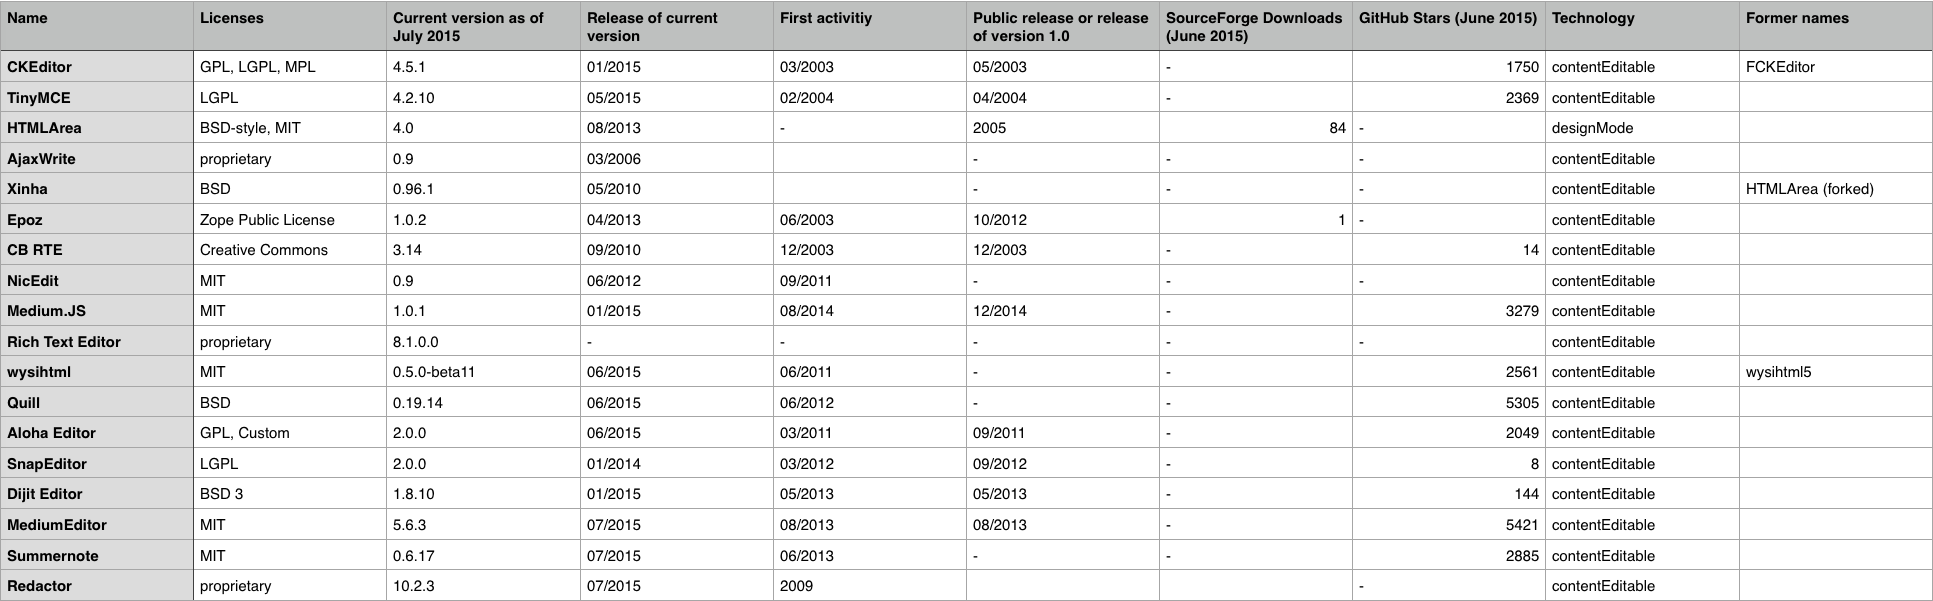
\includegraphics[width=\linewidth]{images/table-ce-editors.png}}
    \caption{Editors using HTML editing APIs (selection)}
    \label{fig:editors_editing_apis_table}
  \end{figure}
  
  \begin{figure}[htb]
    \centerline{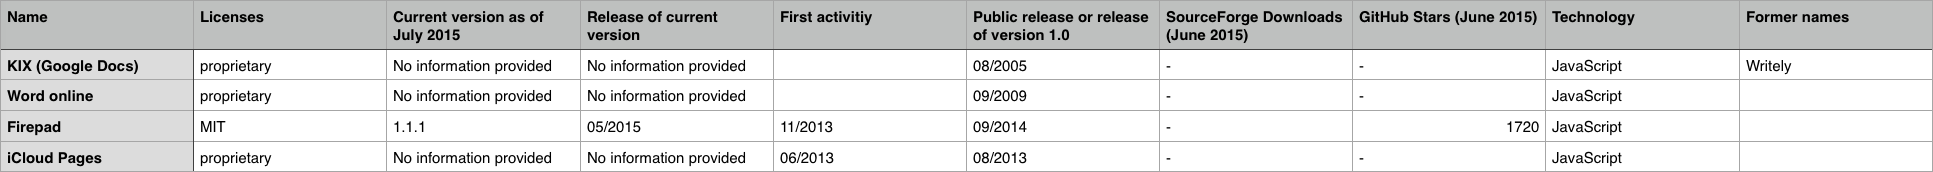
\includegraphics[width=\linewidth]{images/table-js-editors.png}}
    \caption{Editors not using HTML editing APIs (selection)}
    \label{fig:editors_not_editing_apis_table}
  \end{figure}
  
\end{landscape}


\clearpage
\newpage
